\documentclass[14pt]{beamer}
% Možne velikosti pisav so: 8pt, 9pt, 10pt, 11pt, 12pt, 14pt, 17pt, 20pt

% Nastavitve za šumnike
\usepackage[T1]{fontenc}
\usepackage[utf8]{inputenc}
\usepackage[slovene]{babel}

% To potrebujemo, da bomo lahko delali zapiske za predavatelja
\usepackage{pgfpages}

% Treba je ločiti zapiske za predavatelja in prosojnice za občinstvo.
% To lahko naredimo v beamerju, glej
% https://gist.github.com/andrejbauer/ac361549ac2186be0cdb

% Primer tako narejenih prosojnic:
% http://math.andrej.com/wp-content/uploads/2016/06/hott-reals-cca2016.pdf

% Izberemo, ali bomo naredili samo prosojnice, samo zapiske ali oboje

%\setbeameroption{hide notes}                        % samo prosojnice
%\setbeameroption{show only notes}                   % samo zapiski
\setbeameroption{show notes on second screen=right}  % oboje

% Ali naj se \item-i pojavljajo zaporedoma, ali vsi naenkrat?
% Naj se pojavljajo zaporedoma:
% \beamerdefaultoverlayspecification{<+->}

% Minimalistični still
\mode<presentation>
% \usetheme{Goettingen}
% \usecolortheme{rose}

% Malo manj dolgočasna pisava
\usepackage{palatino}
\usefonttheme{serif}

% Izklopimo navigacijske simbole, ker so neuporabni
\setbeamertemplate{navigation symbols}{}

% Aktiviramo oštevilčenje strani
\setbeamertemplate{footline}[frame number]{}

% Stil za zapiske
\setbeamertemplate{note page}{\pagecolor{yellow!5}\insertnote}

\usepackage{amsmath}
\usepackage{amssymb}
\newtheorem{izrek}{Izrek}

\begin{document}

\title{Kako pripravimo prosojnice}
\author{Andrej Bauer}
\date{Planet Zemlja}

\begin{frame}
  \titlepage

  \note[item]{Povej dober vic, da te začnejo poslušati.}
\end{frame}

\begin{frame}
  \frametitle{Zakaj imajo prosojnice naslove?}

  \begin{itemize}
  \item Da predavatelj ve kaj se dogaja.
  \item Ker se predavatelju ne da razmišljati.
  \item Ker je Powerpoint tako naprogramiran.
  \item Tako naštevanje je dolgočasno.
  \end{itemize}


  \note[item]{Tu se delaj norca iz prosojnic z naslovi.}
  \note[item]{Pokritiziraj prosojnice, ki samo nekaj naštevajo.}
  \note[item]{Vprašaj, ali manjka kakšna vejica.}
\end{frame}

\begin{frame}
  \frametitle{Prikažimo vsebino po kosih.}

  \begin{izrek}
    Za vse $x, y \in \mathbb{R}$ velja $x^2 + y^2 \geq 2 x y$.
  \end{izrek}

  \pause

  \begin{proof}
    Vemo, da velja $(x - y)^2 \geq 0$, torej
    %
    \begin{equation*}
      x^2 - 2 x y + y^2 \geq 0.
    \end{equation*}
    %
    \pause
    Ko na obeh straneh prištejemo $2 x y$, dobimo želeno neenačbo
    %
    \begin{equation*}
      x^2 + y^2 \geq 2 x y. \qedhere
    \end{equation*}
  \end{proof}

  \note[item]{Ukaz \texttt{{\char92}pause} vstavi premor v prosojnice.}
  \note[item]{Pojasni, da se ne piše ``željen''.}
\end{frame}

\begin{frame}
  Tu je slika iz interneta:
  %
  \begin{center}
    (Vstavi sliko sem.)
  \end{center}

  \note[item]{Vprašaj, kako se vstavi sliko, da vidimo ali se še spomnijo.}
  \note[item]{Vstavi sliko, pusti študentom, da izberejo vsebino slike, da boš imel boljše študentske ankete.}
  \note[item]{Ne pretiravaj s cinizmom.}
  \note[item]{Vprašaj, v čem je razlika med ironijo in cinizmom.}

\end{frame}


% različni bloki
\begin{frame}{Poudarjeni bloki}

  \begin{exampleblock}{Primer}
    Verjetno ste že opazili, da za naslovno prosojnico niste uporabili
    ukaza \texttt{maketitle}, ampak ukaz \texttt{titlepage}.
  \end{exampleblock}

  \begin{block}{Opomba}
		Okolja za poudarjene bloke so \texttt{block}, \texttt{exampleblock} in \texttt{alertblock}.
	\end{block}
	
	\begin{alertblock}{Pozor!}
		Začetek poudarjenega bloka (ukaz \texttt{begin}) vedno sprejme 
	  dva parametra: okolje in naslov bloka.
	  Drugi parameter (za naslov) je lahko prazen.
	\end{alertblock}
	
\end{frame}


% postopno odkrivanje
\begin{frame}
  \frametitle{Kako se dela pavze}
  Če želimo vsebino postopoma odkrivati
  lahko vstavimo ukaz pause\\
  \pause
  postopno odkrivanje: pause, onslide, only ter določila <…> na ukazih, vključno z <+-> na seznamih
\end{frame}

\begin{frame}
  \frametitle{Onslide}
  \onslide<1->{First Line of Text}
  
  \onslide<2->{Second Line of Text}
  
  \onslide<3->{Third Line of Text}
\end{frame}

\begin{frame}
  \frametitle{Only}
  \only<1>{First Line of Text}
  
  \only<2>{Second Line of Text}
  
  \only<3>{Third Line of Text}
\end{frame}

\begin{frame}{Pavze z znaki<>}
  \text{navaden text}\\
  \texttt<2>{Example text}\\
  \textcolor<3>{orange}{Orange text}
\end{frame}


% več stolpcev v okolju columns in vsak stolpec v okolju column
\begin{frame}
  \frametitle{explanation}
  \begin{columns}
  \begin{column}{0.5\textwidth}
     some text here some text here some text here some text here some text here
  \end{column}
  \begin{column}{0.5\textwidth}  %%<--- here
      \begin{center}
       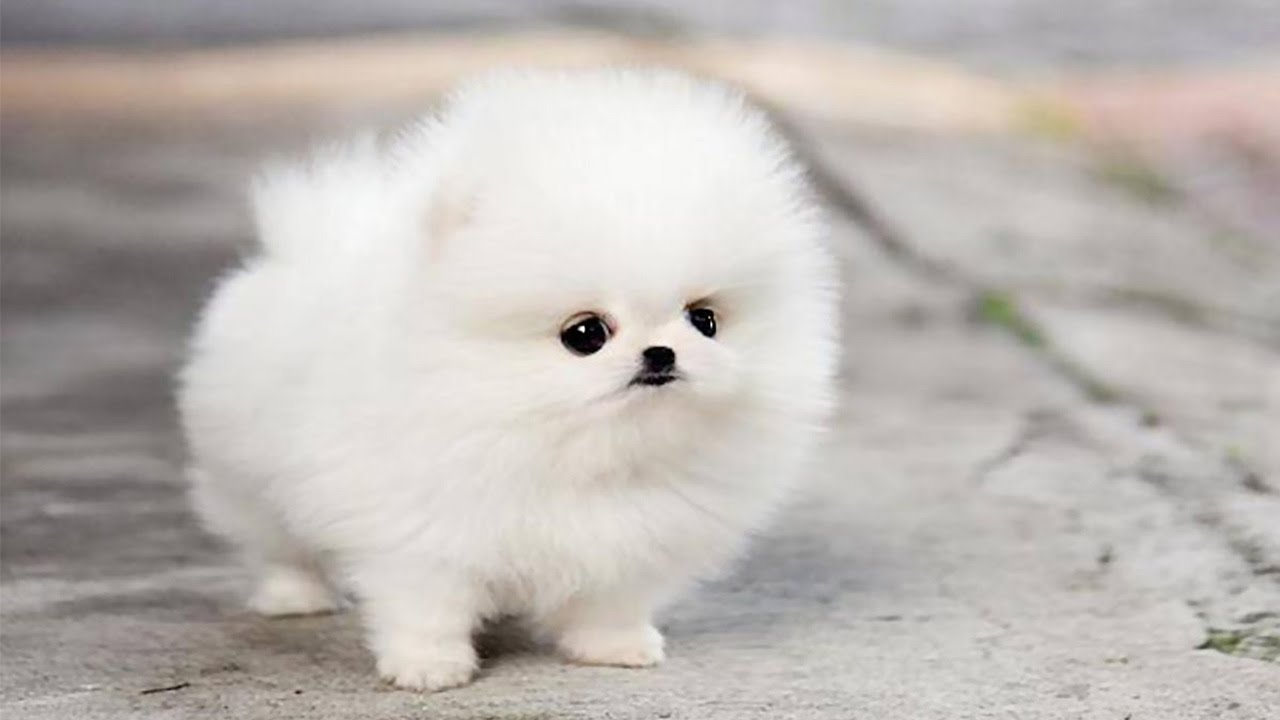
\includegraphics[width=0.8\textwidth]{kuza.jpg}
       \end{center}
  \end{column}
  \end{columns}
\end{frame}



% poveži dva dokumenta
%\section{Stolpci in slike}
%\begin{frame}{Konstrukcija pravokotnice na premico $p$ skozi točko $T$}
	\begin{columns}
		
		\column{0.55\textwidth}
		  \begin{itemize}
			 \item<1-> Dani sta premica $p$ in točka $T$.
			 \item<2-> Nariši lok $k$ s središčem v $T$.
			 \item<3-> Premico $p$ seče v točkah $A$ in $B$.
			 \item<4-> Nariši lok $m$ s središčem v $A$.
			 \item<5-> Nariši lok $n$ s središčem v $B$ in z enakim polmerom.
			 \item<6-> Loka se sečeta v točki $C$.
			 \item<7-> Premica skozi točki $T$ in $C$ je pravokotna na $p$.
		  \end{itemize}

		\column{0.45\textwidth}
		\centering
		  \includegraphics<1>[width=50mm]{slike/fig-1.png}
		  \includegraphics<2>[width=50mm]{slike/fig-2.png}
		  \includegraphics<3>[width=50mm]{slike/fig-3.png}
		  \includegraphics<4>[width=50mm]{slike/fig-4.png}
		  \includegraphics<5>[width=50mm]{slike/fig-5.png}
		  \includegraphics<6>[width=50mm]{slike/fig-6.png}
		  \includegraphics<7>[width=50mm]{slike/fig-7.png}

	\end{columns}

\end{frame}

\begin{frame}{Konstrukcija pravokotnice na premico $p$ skozi točko $T$}
	\begin{columns}
		
		\column{0.55\textwidth}
		  \begin{itemize}
			 \item<1-> Dani sta premica $p$ in točka $T$.
			 \item<2-> Nariši lok $k$ s središčem v $T$.
			 \item<3-> Premico $p$ seče v točkah $A$ in $B$.
			 \item<4-> Nariši lok $m$ s središčem v $A$.
			 \item<5-> Nariši lok $n$ s središčem v $B$ in z enakim polmerom.
			 \item<6-> Loka se sečeta v točki $C$.
			 \item<7-> Premica skozi točki $T$ in $C$ je pravokotna na $p$.
		  \end{itemize}

		\column{0.45\textwidth}
		\centering
		  % Spodnje je za nalogo 3.4.
		    \begin{tikzpicture}
					 % Sliko smo naredili tako, da so točke A, B, T in C vse enako oddaljene
					 % od presečišča premic; kot ATC je 45°.
					 % Vsi krožni loki imajo radij 2.
					 \tikzmath{
					 	% Razdalja od točke T do premice p je tako 2*sin(45°).
					 	\t = 2*sin(45);
					 	% Razdalja začetka loka m do premice p
					 	% oz. razdalja točke T' levo in zgoraj od točke T do premice
					 	\tt = 2*sin(60);
					 	% Razdalja točke T' od navpične premice skozi T
					 	\td = \t-2*cos(60);
					 }
					 % Definicija točke T
					 \coordinate [label={[blue, above left]:$T$}] (T) at (0,{\t});
					 % Risanje točke T
					 \fill[blue] (T) circle (2pt);
					 % Premica p
					 \draw[blue, very thick] (-2,0) -- (2,0) node[right] {$p$};
					 \pause
					 % Definicija pomožne točke A' in risanje krožnega loka k, ki se začne v A'
					 \coordinate (A') at ({-\tt},{\td});
					 \draw[gray, thin] (A') arc[start angle=210, end angle=330, radius=2] node[right] {\scriptsize $k$};
					 \pause
					 % Točka A
					 \coordinate [label=below left:{\scriptsize $A$}] (A) at ({-\t},0);
					 \draw (A) circle (1.5pt);
					
					 % Naloga 3.4.1.: Narišite še točko B (skupaj z oznako)
					 \coordinate [label=below right:{\scriptsize $B$}] (B) at ({\t},0);
					 \draw (B) circle (1.5pt);
					 \pause
					 % Naloga 3.4.2.: Definirajte točko T', v kateri se začne lok m in narišite lok m z oznako.
					 % Lok je definiran s točko, v kateri se lok začne (ne središče!), z začetnim in končnim kotom ter radijem.
					 % Koti so vedno podani enako: kot 0 je v smeri x osi in se veča v nasprotni smeri urinega kazalca.
					 \coordinate (T') at ({-\td},{\tt});
					 \draw[gray, thin] (T') arc[start angle=60, end angle=-60, radius=2] node[right] {\scriptsize $m$};	
					 \pause
					 % Naloga 3.4.3.: Definirajte točko T'' in narišite lok n z oznako.
					 \coordinate (T') at ({\td},{\tt});
					 \draw[gray, thin] (T') arc[start angle=120, end angle=240, radius=2] node[right] {\scriptsize $n$};	
					 \pause
					 % Naloga 3.4.4.: Definirajte in narišite točko C.	
					 \coordinate [label=below right:{\scriptsize $C$}] (C) at ({0},{-\t});
					 \draw (C) circle (1.5pt);
					 \pause
					 % Naloga 3.4.5.: Narišite premico skozi točki T in C.
					 \draw[red, very thick] (0,-2) -- (0,2) node[right] {$$};
			\end{tikzpicture}

				% Konec vsebine za nalogo 3.4.

	\end{columns}

\end{frame}



% Naloga 4
\begin{frame}{Graf funkcije s TikZ}
	\centering
	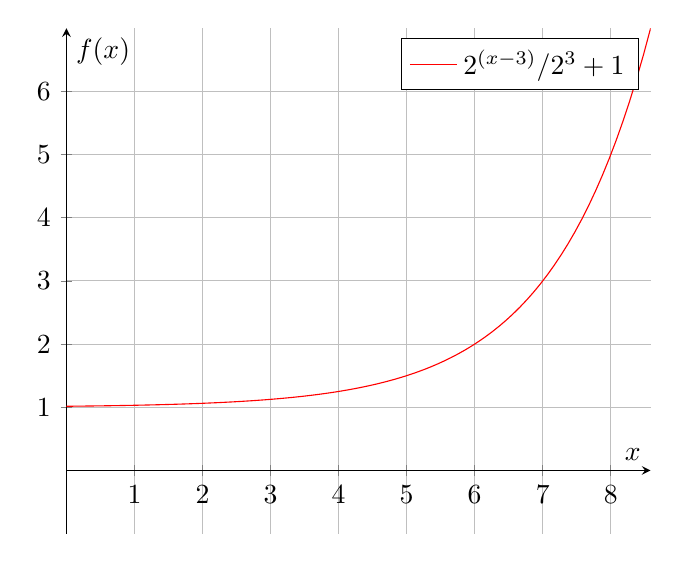
\begin{tikzpicture}
		\begin{axis}[
			axis lines = middle,
			domain = 0:10,
			width = 9cm,
			height = 8cm,
			xtick = {0, 1, 2, 3, 4, 5, 6, 7, 8},
			ytick = {0, 1, 2, 3, 4, 5, 6},
			ymin = -1,
			ymax = 7,
			grid = both,
			xlabel = {$x$},
			ylabel = {$f(x)$}
		]
		\addplot [
    	domain=-0:10, 
    	samples=100, 
    	color=red,
		]
		{2^(x - 3)/2^3 + 1};
		\addlegendentry{\(2^{(x - 3)}/2^3 + 1\)}
		\end{axis}
	\end{tikzpicture}
\end{frame}

\end{document}
